\chapter{Near the Horizon of a Schwarzschild Black Hole}

Before setting out on the advertised journey into a large black hole, Leonard Susskind rewinds. He wants one more pass through the accelerated frame, because the whole near-horizon story is already hiding there in simpler form. So we begin where the lecture begins: with hyperbolic motion in flat spacetime, then with the question of what Alice and Bob actually see, and only then with the Schwarzschild metric itself. From there the chapter follows the lecture step by step: what looks singular, what is only a coordinate artifact, how the near-horizon metric becomes Rindler, why the horizon is locally innocuous but causally decisive, and finally where the metric comes from in Einstein’s equations. These notes follow Leonard Susskind’s lecture, with the surviving board evidence preserved here through the archival curation of LazyingArt LLC and Video2Book.

\section{Accelerated Observers and Hyperbolic Coordinates}

Before talking about black holes, Susskind goes back to the accelerated reference frame and reminds us what was special about it. The important point is that this is not merely a formal change of variables. We first rewrite Minkowski space in unusual coordinates, and then we imagine a family of observers who remain at fixed values of the new spatial coordinate. Those fixed-coordinate observers are the accelerated observers.

On the board Susskind writes \(x\) and \(t\). To keep them separate from the Schwarzschild time \(t\) that will appear shortly, we will write the local flat-space coordinates as \((X,T)\). The hyperbolic coordinate map is
\begin{equation}
X=r\cosh\omega,
\qquad
T=r\sinh\omega.
\end{equation}
This is the timelike analog of polar coordinates. In ordinary Euclidean geometry one writes \(x=r\cos\theta\), \(y=r\sin\theta\); here the circular angle is replaced by the hyperbolic angle \(\omega\).

From the map we immediately obtain
\begin{equation}
X^2-T^2=r^2,
\qquad
\frac{T}{X}=\tanh\omega.
\end{equation}
Thus the curves of constant \(r\) are hyperbolae, while the curves of constant \(\omega\) are rays through the origin. The closer a constant-\(r\) curve lies to the light cone, the tighter it turns, and the larger the acceleration required to keep an observer on it. This is why the accelerated frame is not a Newtonian ``rigidly accelerated'' frame in which everybody shares the same acceleration. The acceleration varies from one worldline to another.

Now let us write the metric. In Minkowski coordinates,
\begin{equation}
d\tau^2=dT^2-dX^2-dy^2-dz^2.
\end{equation}
Substituting the hyperbolic coordinates gives
\begin{equation}
d\tau^2=r^2\,d\omega^2-dr^2-dy^2-dz^2.
\end{equation}
Along a fixed-\(r\) trajectory, with \(dr=dy=dz=0\), this becomes
\begin{equation}
d\tau=r\,d\omega.
\end{equation}
This is one of the clarifications Susskind insists on in the lecture. The coordinate \(\omega\) is not everybody’s proper time. It is a common time label for the accelerated frame, but clocks sitting at different \(r\) tick proper time at different rates. If one insists on building clocks that all read \(\omega\), then those clocks must be adjusted differently from one hyperbola to another.

This is also where he pauses over a possible misunderstanding. The map \((X,T)\mapsto(r,\omega)\) is indeed just a coordinate transformation. The physical content enters when we populate the fixed-\(r\) curves with observers and ask what those observers see. A coordinate change by itself does not create acceleration; the acceleration comes from the decision to hold observers on the constant-\(r\) hyperbolae.

\begin{figure}[htbp]
\centering
\includegraphics[width=0.78\textwidth]{lecture_12_figure_02.png}

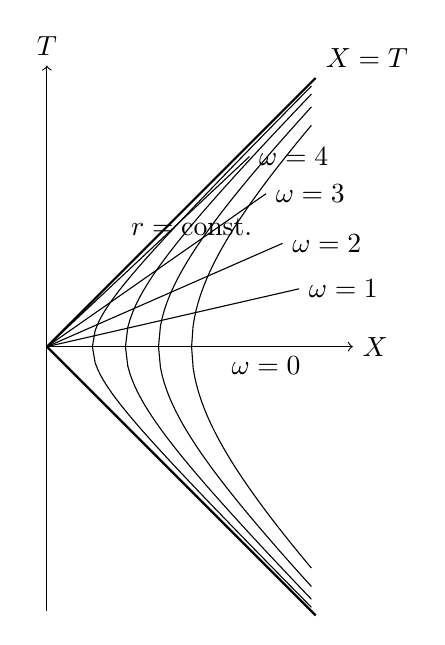
\begin{tikzpicture}[scale=1.05]
\draw[->] (0,-3.2) -- (0,3.4) node[above] {$T$};
\draw[->] (0,0) -- (3.7,0) node[right] {$X$};
\draw[thick] (0,0) -- (3.25,3.25) node[above right] {$X=T$};
\draw[thick] (0,0) -- (3.25,-3.25);

\draw[domain=0.55:3.2,samples=80] plot (\x,{sqrt(\x*\x-0.55*0.55)});
\draw[domain=0.55:3.2,samples=80] plot (\x,{-sqrt(\x*\x-0.55*0.55)});
\draw[domain=0.95:3.2,samples=80] plot (\x,{sqrt(\x*\x-0.95*0.95)});
\draw[domain=0.95:3.2,samples=80] plot (\x,{-sqrt(\x*\x-0.95*0.95)});
\draw[domain=1.35:3.2,samples=80] plot (\x,{sqrt(\x*\x-1.35*1.35)});
\draw[domain=1.35:3.2,samples=80] plot (\x,{-sqrt(\x*\x-1.35*1.35)});
\draw[domain=1.75:3.2,samples=80] plot (\x,{sqrt(\x*\x-1.75*1.75)});
\draw[domain=1.75:3.2,samples=80] plot (\x,{-sqrt(\x*\x-1.75*1.75)});

\draw (0,0) -- (3.2,0);
\draw (0,0) -- (3.05,0.7);
\draw (0,0) -- (2.85,1.25);
\draw (0,0) -- (2.65,1.85);
\draw (0,0) -- (2.45,2.3);

\node[below] at (2.65,0) {$\omega=0$};
\node[right] at (3.05,0.7) {$\omega=1$};
\node[right] at (2.85,1.25) {$\omega=2$};
\node[right] at (2.65,1.85) {$\omega=3$};
\node[right] at (2.45,2.3) {$\omega=4$};
\node at (1.75,1.45) {$r=\mathrm{const.}$};
\end{tikzpicture}
\caption{Rindler wedge and the \((r,\omega)\) coordinate map. The screenshot is kept because it preserves the original board layout and labels, while the redraw makes the geometry clean.}
\end{figure}

The line \(X=T\) is the limiting horizon of the accelerated coordinates. The ray \(\omega=0\) is the slice \(T=0\), and as \(\omega\to\infty\), the constant-\(\omega\) rays pile up against the lightlike boundary \(X=T\). In this coordinate system the horizon is reached only at the end of accelerated time.

\section{Alice, Bob, and the Horizon as a Visual Limit}

Once the geometry is back on the board, the lecture pivots from coordinates to observation. The natural question is no longer only ``what are the curves?'', but ``what does an observer see?'' Susskind immediately reminds us that seeing means receiving light, and therefore seeing always involves looking backward along null lines.

Let Alice fall freely across the horizon while Bob remains supported outside, riding one of the accelerated worldlines. Bob sees Alice by tracing past-directed light rays from his own trajectory. At one moment he receives light emitted from one point on Alice’s path, a little later from a point closer to the horizon, and later still from a point closer still. In Bob’s description Alice never crosses the horizon in finite accelerated time. She asymptotically approaches it.

This is already enough to understand why Bob says that Alice freezes. Her clock appears to slow, her emitted signals arrive farther and farther apart, and in the geometrical picture she is squeezed closer and closer to the limiting null line.

Alice, however, reports nothing of that sort locally. She simply falls through. If she looks back, she does not see Bob vanish. She sees Bob receding away on an accelerated trajectory. So there is an asymmetry here, but it is an asymmetry in the structure of signals, not a local physical singularity at the horizon.

\begin{figure}[htbp]
\centering
\includegraphics[width=0.82\textwidth]{lecture_12_figure_04.png}

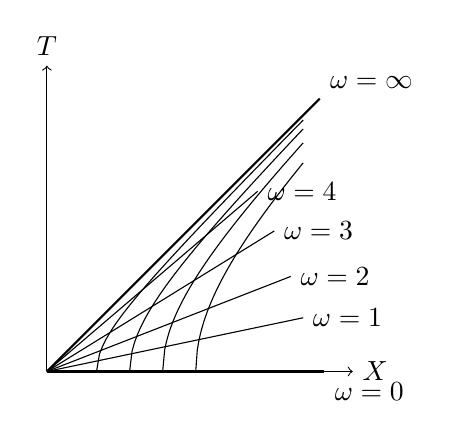
\begin{tikzpicture}[scale=1.05]
\draw[->] (0,0) -- (3.7,0) node[right] {$X$};
\draw[->] (0,0) -- (0,3.7) node[above] {$T$};
\draw[thick] (0,0) -- (3.3,3.3) node[above right] {$\omega=\infty$};
\draw[very thick] (0,0) -- (3.35,0) node[below right] {$\omega=0$};
\draw (0,0) -- (3.1,0.65);
\draw (0,0) -- (2.95,1.15);
\draw (0,0) -- (2.75,1.7);
\draw (0,0) -- (2.55,2.18);

\draw[domain=0.6:3.1,samples=70] plot (\x,{sqrt(\x*\x-0.6*0.6)});
\draw[domain=1.0:3.1,samples=70] plot (\x,{sqrt(\x*\x-1.0*1.0)});
\draw[domain=1.4:3.1,samples=70] plot (\x,{sqrt(\x*\x-1.4*1.4)});
\draw[domain=1.8:3.1,samples=70] plot (\x,{sqrt(\x*\x-1.8*1.8)});

\node[right] at (3.1,0.65) {$\omega=1$};
\node[right] at (2.95,1.15) {$\omega=2$};
\node[right] at (2.75,1.7) {$\omega=3$};
\node[right] at (2.55,2.18) {$\omega=4$};
\end{tikzpicture}
\caption{Constant-\(\omega\) lines piling up at the horizon. This is the visual content of the statement that nothing reaches the horizon at finite \(\omega\).}
\end{figure}

\subsection{Question \& Answer}

\paragraph{Question.} Why does Bob see asymptotic freezing while Alice notices no special event at the horizon?

\paragraph{Answer.} Because the two observers are not using the same family of clocks and not sampling the same family of light rays. Bob remains supported outside and uses the accelerated time variable \(\omega\). For him the horizon sits at \(\omega=\infty\). Each light signal he receives from Alice was emitted from a point closer to that limiting line, so her clock appears to slow more and more.

Alice is freely falling. Near the horizon the local geometry is smooth, and in her own proper time the crossing occurs after a finite interval. She can look back and see Bob receding, and she can see his processes slowed by recession, but she does not encounter a local catastrophe at the horizon itself. The freezing is therefore not evidence that the horizon is a physical wall. It is evidence that Bob’s outside description uses a time coordinate for which the horizon lies infinitely far away.

This same point reappears later in black-hole language. Two freely falling observers can continue to exchange signals in the ordinary way as long as the causal structure permits it. The sharp one-way barrier arises between the infalling observer and the observer who chooses not to fall, that is, the observer who remains supported outside.

\section{The Schwarzschild Metric and Its Suspicious Radii}

With the accelerated picture in place, Susskind makes the day’s main transition explicit: now he wants to connect that picture to the Schwarzschild metric. Once we know the connection, he says, many questions about black holes can be answered by thinking through the corresponding accelerated-frame question.

The Schwarzschild line element is
\begin{equation}
d\tau^2
=
\left(1-\frac{2MG}{r}\right)dt^2
-
\frac{dr^2}{1-\frac{2MG}{r}}
-
r^2\,d\Omega^2,
\qquad
d\Omega^2=d\theta^2+\sin^2\theta\,d\phi^2.
\end{equation}
This is the metric outside any spherically symmetric mass distribution. In particular, it is also the metric outside the Earth, outside a star, or outside any collapsed body, provided we stay outside the region where the matter itself is located.

\begin{figure}[htbp]
\centering
\includegraphics[width=0.82\textwidth]{lecture_12_figure_03.png}
\caption{Schwarzschild line element written on the board. The left edge is cropped, so the displayed equation above gives the clean standard reconstruction.}
\end{figure}

Immediately two suspicious radii appear:
\begin{equation}
r=2MG,
\qquad
r=0.
\end{equation}
At \(r=2MG\), the coefficient of \(dt^2\) goes to zero and the coefficient of \(dr^2\) blows up. At \(r=0\), the coefficients do something even more violent, and the sign pattern changes. The lecture’s next move is not yet to solve the problem, but to sharpen it. Which of these pathologies are real, and which are artifacts of coordinates?

Before answering, Susskind manufactures the same sort of pathology in flat spacetime. This is the warning example that keeps the later black-hole calculation honest.

At this point he abandons the old accelerated-frame notation \(r\), because Schwarzschild \(r\) is now on stage. Let us therefore rename the accelerated radial variable \(\rho\). On the board the lecturer introduces a new auxiliary variable and simply calls it \(R\). To keep it separate from the Ricci scalar that will appear later, let us call it
\begin{equation}
R_{\mathrm{aux}}=\rho^2.
\end{equation}
Then
\begin{equation}
dR_{\mathrm{aux}}=2\rho\,d\rho,
\qquad
d\rho^2=\frac{dR_{\mathrm{aux}}^2}{4R_{\mathrm{aux}}}.
\end{equation}
The flat accelerated metric
\begin{equation}
d\tau^2=\rho^2\,d\omega^2-d\rho^2-dy^2-dz^2
\end{equation}
can now be rewritten as
\begin{equation}
d\tau^2
=
R_{\mathrm{aux}}\,d\omega^2
-
\frac{dR_{\mathrm{aux}}^2}{4R_{\mathrm{aux}}}
-
dy^2
-
dz^2.
\end{equation}
Here the same pattern appears: one coefficient vanishes where the other diverges. But spacetime is still perfectly flat. Nothing singular has happened physically. The pathology lies in the coordinates, not in the geometry.

The continuation across the horizon is also transparent in this toy model. Since
\begin{equation}
X^2-T^2=\rho^2=R_{\mathrm{aux}},
\end{equation}
the region \(R_{\mathrm{aux}}<0\) is simply the region where
\begin{equation}
T^2-X^2=-R_{\mathrm{aux}}.
\end{equation}
So the sign flip does not mean that spacetime itself has become pathological. It means that the same coordinate symbol is now labeling a different family of curves.

That is the diagnostic lesson Susskind wants in hand before returning to the black hole. One can have a vanishing coefficient, an infinite coefficient, and even an exchange of timelike and spacelike character in the coordinates without any local catastrophe.

By contrast, the lecture also insists that \(r=0\) in Schwarzschild is different. There the singularity is not merely a failure of coordinates. Tidal forces diverge there. The geometry itself is singular.

\section{Near the Horizon: From Schwarzschild to Rindler}

Now comes the constructive core of the lecture. Can we actually see the Schwarzschild metric becoming the accelerated-frame metric near the horizon? If we can, then we will know that the horizon is locally no more singular than the Rindler horizon in flat spacetime.

Let us begin by rewriting the Schwarzschild factor:
\begin{equation}
1-\frac{2MG}{r}=\frac{r-2MG}{r}.
\end{equation}
Accordingly,
\begin{equation}
d\tau^2
=
\frac{r-2MG}{r}\,dt^2
-
\frac{r}{r-2MG}\,dr^2
-
r^2\,d\Omega^2.
\end{equation}

Now let us say clearly what approximation is being made. We are not approximating the whole black hole. We are examining a small neighborhood of one chosen point on the horizon. The quantity \(r-2MG\) may be small and may even change sign, so we keep it explicit. But the slowly varying factor \(r\) itself changes very little in a tiny neighborhood of the horizon, so in those places we may set \(r\approx 2MG\). This gives
\begin{equation}
d\tau^2
\approx
\frac{r-2MG}{2MG}\,dt^2
-
\frac{2MG}{r-2MG}\,dr^2
-
(2MG)^2\,d\Omega^2.
\end{equation}

The angular term is still the metric on a two-sphere of radius \(2MG\). But in the immediate vicinity of one point on that sphere, the sphere looks like its tangent plane. So the lecture replaces the angular metric by a flat patch:
\begin{equation}
(2MG)^2\,d\Omega^2 \approx dy^2+dz^2.
\end{equation}
The local near-horizon metric therefore becomes
\begin{equation}
d\tau^2
\approx
\frac{r-2MG}{2MG}\,dt^2
-
\frac{2MG}{r-2MG}\,dr^2
-
dy^2
-
dz^2.
\end{equation}

At this point Susskind stops and tells us what he is doing. He is looking at the horizon under a microscope. The whole purpose of the calculation is to decide whether the horizon is locally nasty or locally tame.

The next move is the decisive one. We introduce a new coordinate \(\rho\), defined to be the proper spatial distance from the horizon. If we move purely in the radial direction, keeping \(t\), \(y\), and \(z\) fixed, then the proper distance element is determined by the radial part of the metric:
\begin{equation}
d\rho^2=\frac{2MG}{r-2MG}\,dr^2.
\end{equation}
This is not an accident and not a guess. It is chosen precisely so that the awkward radial term becomes the simple flat-space term \(-d\rho^2\).

Now integrate. The proper distance from the horizon \(r=2MG\) to an outside point \(r\) is
\begin{align}
\rho
&=
\int_{2MG}^{r}\sqrt{\frac{2MG}{r'-2MG}}\,dr' \\
&=
2\sqrt{2MG}\,\sqrt{r-2MG} \\
&=
\sqrt{8MG}\,\sqrt{r-2MG}.
\end{align}
So we can invert the relation:
\begin{equation}
r-2MG=\frac{\rho^2}{8MG}.
\end{equation}
Substitute this into the coefficient of \(dt^2\):
\begin{equation}
\frac{r-2MG}{2MG}\,dt^2
=
\frac{\rho^2}{16M^2G^2}\,dt^2.
\end{equation}
The metric becomes
\begin{equation}
d\tau^2
=
\frac{\rho^2}{16M^2G^2}\,dt^2
-
d\rho^2
-
dy^2
-
dz^2.
\end{equation}

We are almost done. There is only one mismatch with the Rindler form, namely the harmless factor \(16M^2G^2\) in the time term. Remove it by rescaling time:
\begin{equation}
\omega=\frac{t}{4MG},
\qquad
d\omega=\frac{dt}{4MG}.
\end{equation}
Then the metric is
\begin{equation}
d\tau^2
=
\rho^2\,d\omega^2
-
d\rho^2
-
dy^2
-
dz^2.
\end{equation}
This is exactly the accelerated-frame metric.

\begin{figure}[htbp]
\centering
\includegraphics[width=0.72\textwidth]{lecture_12_figure_05.png}
\caption{Near-horizon Rindler-form metric and time rescaling. The board image is kept because it shows the metric block and the redraw setup coexisting at the same moment in the lecture.}
\end{figure}

That is the bridge the lecture wanted to build. Near one point on the horizon, and for a sufficiently small neighborhood, the Schwarzschild metric is the Rindler metric. The horizon is not a local curvature singularity. It is flat spacetime in strange coordinates, just as the accelerated frame was.

\section{What the Horizon Does and Does Not Mean}

Once the metric match is in hand, the lecture cashes it out physically. The horizon is not a place where local geometry blows up. But it is still a very special surface, because it separates what can and cannot communicate with the outside.

A fixed Schwarzschild radius \(r>2MG\) corresponds to a supported observer, not a freely falling one. Near the horizon, such an observer is the black-hole analog of the accelerated observer in flat spacetime. This is why the outside description inherits all the same features: the horizon is reached only at infinite outside time, and something falling in appears to freeze, slow, and redden.

The redshift discussion in the lecture is particularly concrete. Susskind imagines Alice falling inward while emitting a steady sequence of light crests in her own proper time. Bob, supported outside, receives those crests farther and farther apart in his own proper time. The first crests arrive as ordinary light, then as longer and longer wavelengths, then infrared, then microwave, then radio waves of absurdly large wavelength. In that sense there is a ``last wave'' of any finite-frequency process. Bob sees not only Alice’s clock, but everything about Alice, slow down and redshift away.

This is why the lecture repeatedly says that Bob never sees Alice cross the horizon. What Bob sees is matter piling up closer and closer to the horizon, merging with it from the outside description. The black hole grows not because Bob sees something neatly cross a sharp boundary, but because the horizon itself grows to include the infalling energy.

There is a corresponding statement about communication. Two freely falling observers behave ordinarily with respect to one another so long as the causal structure allows it. If one observer, Shirley, freely falls after Alice, the two can continue to exchange signals in the ordinary way until the interior geometry forbids it. But if Shirley changes her mind at the last moment and remains supported outside, then Alice drops out of Shirley’s experience once Alice has crossed the horizon. That asymmetry is the black-hole version of the earlier Alice-and-Bob accelerated-frame story.

The lecture also addresses a more geometric question: can one skim sideways along the horizon? The answer is no. Near the horizon, if one insists on holding \(r\) fixed and sets \(dr=0\), then
\begin{equation}
d\tau^2
\approx
\frac{r-2MG}{2MG}\,dt^2-dy^2-dz^2.
\end{equation}
Now let \(r\) be extremely close to \(2MG\). The coefficient of \(dt^2\) becomes arbitrarily small. A finite transverse excursion in \(y\) or \(z\) then overwhelms the timelike term and makes the interval spacelike. In other words, a would-be trajectory that ``skirts the horizon'' at fixed \(r\) becomes faster than light. That is forbidden. One may stay outside, or one may cross inward, but one cannot ride the horizon sideways.

So the horizon is not singular, but it is the boundary of no return for supported observers. That is the precise sense in which it is special.

\section{Inside the Horizon and the Nature of the Singularity}

Now the lecture turns from the horizon to the genuine singularity. The question is no longer whether \(r=2MG\) is harmless. We have already seen that it is. The question is where \(r=0\) sits in the geometry, and why it is impossible to avoid once one has crossed the horizon.

For \(r<2MG\),
\begin{equation}
1-\frac{2MG}{r}<0.
\end{equation}
So the coefficient of \(dt^2\) becomes negative and the coefficient of \(dr^2\) becomes positive. Susskind is very careful here: this does not mean that space itself has somehow literally turned into time. It means that these coordinates have been continued past a horizon, and their timelike and spacelike roles have exchanged in much the same way as in the flat-space toy model with \(R_{\mathrm{aux}}<0\).

That toy model already told us what to expect. Outside the Rindler horizon we had
\begin{equation}
X^2-T^2=R_{\mathrm{aux}}>0,
\end{equation}
so fixed \(R_{\mathrm{aux}}\) gave timelike hyperbolae in the right wedge. Inside, where \(R_{\mathrm{aux}}<0\), the same equation becomes
\begin{equation}
T^2-X^2=-R_{\mathrm{aux}},
\end{equation}
and fixed \(R_{\mathrm{aux}}\) now labels spacelike hyperbolae in the upper quadrant. That is the flat-space model of what happens to fixed Schwarzschild \(r\) inside the black hole. Outside, fixed \(r\) can describe a supported observer. Inside, fixed \(r\) is no longer a possible timelike worldline; it is a spacelike slice.

This is the content of Susskind’s phrase that fixed \(r\) inside is ``some time, not some place.'' One should hear it geometrically, not mystically. Inside the horizon, constant Schwarzschild \(r\) does not describe where a static observer sits. It describes a future-directed slicing of the interior.

\begin{figure}[htbp]
\centering
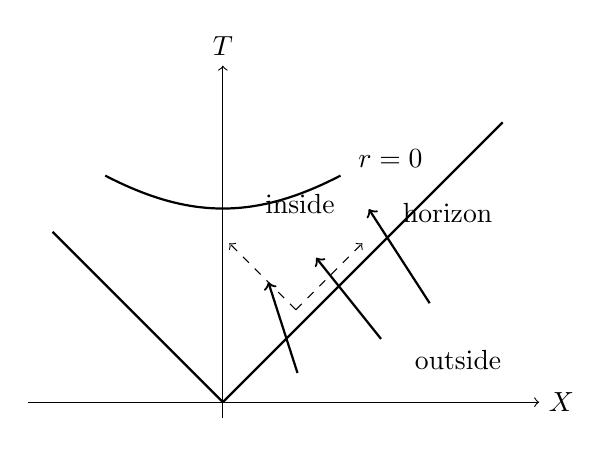
\begin{tikzpicture}[scale=1.03]
\draw[->] (-2.4,0) -- (3.9,0) node[right] {$X$};
\draw[->] (0,-0.2) -- (0,4.15) node[above] {$T$};

\draw[thick] (0,0) -- (3.45,3.45);
\draw[thick] (0,0) -- (-2.1,2.1);

\draw[thick,domain=-1.45:1.45,samples=120] plot (\x,{sqrt(\x*\x+5.7)});
\node[right] at (1.55,3.0) {$r=0$};

\draw[->,thick] (1.95,0.78) -- (1.15,1.78);
\draw[->,thick] (2.55,1.22) -- (1.8,2.38);
\draw[->,thick] (0.92,0.36) -- (0.56,1.48);

\draw[->,dashed] (0.9,1.14) -- (1.72,1.96);
\draw[->,dashed] (0.9,1.14) -- (0.08,1.96);

\node at (2.9,0.52) {outside};
\node at (0.95,2.45) {inside};
\node[above right] at (2.1,2.1) {horizon};
\end{tikzpicture}
\caption{A causal redraw of the interior picture. The singularity \(r=0\) is a spacelike future boundary, not a point that one might steer around.}
\end{figure}

This is why the singularity is not best thought of as a place. If it were only a point sitting somewhere inside, one could imagine missing it. But that is not the geometry. In the causal picture the singularity is a spacelike future boundary. Once one falls through the horizon, every future-directed timelike or lightlike trajectory ends there. Even an ``outgoing'' light ray inside still moves toward the singularity in the causal diagram.

\subsection{Question \& Answer}

\paragraph{Question.} Is the singularity a place one could try to avoid, or is it a future spacelike boundary that one inevitably reaches after crossing the horizon?

\paragraph{Answer.} The lecture’s answer is that the singularity is not a place in the ordinary Newtonian sense. If it were merely a point in space, one might hope to go around it. But once the interior geometry is drawn correctly, \(r=0\) is a spacelike future boundary. Inside the horizon, both inward-going and outward-going null rays hit it, and therefore every future-directed timelike or null trajectory reaches it in finite proper time.

This is the sharp contrast with the horizon. The horizon is locally uneventful but globally decisive. The singularity is globally unavoidable and locally catastrophic. The lecturer sometimes calls it ``the end of time,'' but the cleaner statement is that once the horizon has been crossed, only a finite amount of proper time remains before the classical trajectory terminates at \(r=0\).

This is also the place where Susskind adds an important physical qualification. For a stellar-mass black hole, the tidal forces at the horizon are already severe enough to destroy an ordinary human observer. For a sufficiently large black hole, however, the horizon is so large and so nearly flat that one can pass through it without appreciable local distress. The real violence then occurs later, at the singularity, not at the horizon. Crossing the horizon is not the dangerous event; it is the event after which doom becomes unavoidable.

Late in the lecture Susskind pushes the story one step further and asks what happens to matter near the singularity. His description there is heuristic rather than part of the main derivation: as one approaches the singularity, different parts of an object lose causal contact with one another, first at the scale of ordinary matter and then at smaller scales. That imagery is valuable for intuition, but the central classical statement is already complete without it. The singularity is the genuine curvature catastrophe, and nothing survives to report back from it.

\section{Vacuum Field Equations, Exterior Solutions, and Why Black Holes Form}

Late in the lecture a student asks to go back to the source of the metric. That question changes the tone. We step away from the horizon geometry and return to Einstein’s equations themselves.

Outside the matter distribution there is no local source. In that exterior region Einstein’s equations reduce to the vacuum equations
\begin{equation}
R_{\mu\nu}-\frac{1}{2}g_{\mu\nu}R=0.
\end{equation}
This is the relativistic analog of the Newtonian statement that outside the source the potential satisfies Laplace’s equation:
\begin{equation}
\nabla^2\phi=\rho_{\mathrm{mass}},
\qquad
\nabla^2\phi=0
\quad \text{outside matter.}
\end{equation}

\begin{figure}[htbp]
\centering
\includegraphics[width=0.68\textwidth]{lecture_12_figure_06.png}
\caption{Vacuum Einstein equation and Newtonian Poisson analogy. The board’s lower source term is schematic, so the typeset equations here give the normalized notation.}
\end{figure}

The lecture then asks for the radially symmetric Newtonian solution. If \(\phi=\phi(R)\) depends only on the radial distance \(R\), Laplace’s equation becomes
\begin{equation}
\frac{1}{R^2}\frac{d}{dR}\!\left(R^2\frac{d\phi}{dR}\right)=0.
\end{equation}
Integrating once gives
\begin{equation}
R^2\frac{d\phi}{dR}=C,
\end{equation}
and integrating again,
\begin{equation}
\phi(R)=-\frac{C}{R}+\text{constant}.
\end{equation}
If we require \(\phi\to 0\) at infinity, the additive constant vanishes, and the remaining constant is fixed by the enclosed mass. Thus
\begin{equation}
\phi(R)=-\frac{GM}{R}.
\end{equation}
This is exactly the analogy Susskind wants. Outside the source, symmetry plus the field equation fixes the form of the exterior solution.

He then uses that comparison to explain why Einstein’s old intuition about black holes was wrong. In Newtonian mechanics a point singularity is a point in space. A particle thrown toward it will generally miss unless aimed with absurd precision; a little angular momentum is enough to send it past. That is why in ordinary classical mechanics a generic cloud of particles does not collapse to a literal point. Einstein carried some version of that intuition over to gravitation and thought black holes could not really form.

But the black-hole singularity is not a point one might miss after the horizon has formed. Once the horizon is crossed, the singularity lies to the future. The horizon is the surface of no return, and beyond it all future-directed motion ends at \(r=0\). That is the conceptual mistake in the Newtonian analogy. The black-hole singularity is not merely a target in space. It is a future boundary in spacetime.

There is also a simple scaling argument for why black holes can form even when the average density is small. Let a ball of matter have mass \(M\), radius \(R\), and mean density \(\bar\rho\). Then, up to numerical factors,
\begin{equation}
M\sim \bar\rho\,R^3,
\qquad
R\sim\left(\frac{M}{\bar\rho}\right)^{1/3}.
\end{equation}
The Schwarzschild radius is
\begin{equation}
R_{\mathrm S}=2GM.
\end{equation}
Now compare the two scalings at fixed \(\bar\rho\). The size of the ball grows like \(M^{1/3}\), while the Schwarzschild radius grows like \(M\). Therefore, for sufficiently large \(M\),
\begin{equation}
R_{\mathrm S}>R.
\end{equation}
That is exactly the black-hole condition. No matter how small the mean density is, if one takes enough mass, the Schwarzschild radius eventually outgrows the ordinary radius of the matter distribution. This is the robust conclusion at the end of the lecture: larger black holes can form at lower average density. Black-hole formation is therefore not blocked by the naive classical thought that matter ought simply to miss a central point.

\section{Summary}

The lecture begins by delaying the plunge into the black hole and returning to the accelerated frame. That rewind is essential. The near-horizon region of a Schwarzschild black hole is locally the Rindler wedge, and the metric near one point on the horizon becomes
\begin{equation}
d\tau^2=\rho^2\,d\omega^2-d\rho^2-dy^2-dz^2.
\end{equation}
This shows that \(r=2MG\) is not a local curvature singularity.

But the horizon is still special. For supported observers it is the limit of no return. Outside observers assign infinite coordinate time to crossing, see infalling matter slow and redden, and never see a finite-time crossing of the horizon. None of that means the horizon is a physical wall; it means only that the outside coordinates are singular there.

The real singularity is at \(r=0\). Inside the horizon, fixed Schwarzschild \(r\) becomes spacelike, and the singularity is a spacelike future boundary rather than an ordinary place. Once the horizon is crossed, every future-directed timelike or null trajectory ends there in finite proper time. Finally, outside matter the metric is governed by the vacuum Einstein equation, just as the Newtonian potential outside sources satisfies Laplace’s equation. The exterior field is determined by the enclosed mass, and the scaling of the Schwarzschild radius shows why sufficiently large masses form black holes even at very low average density.